\let\negmedspace\undefined
\let\negthickspace\undefined
\documentclass[journal,12pt,onecolumn]{IEEEtran}
\usepackage{cite}
\usepackage{amsmath,amssymb,amsfonts,amsthm}
\usepackage{algorithmic}
\usepackage{graphicx}
\graphicspath{{Figs/}}
\usepackage{textcomp}
\usepackage{xcolor}
\usepackage{txfonts}
\usepackage{listings}
\usepackage{enumitem}
\usepackage{mathtools}
\usepackage{gensymb}
\usepackage{comment}
\usepackage{caption}
\usepackage[breaklinks=true]{hyperref}
\usepackage{tkz-euclide} 
\usepackage{listings}
\usepackage{gvv}                                        
%\def\inputGnumericTable{}                                 
\usepackage[latin1]{inputenc}     
\usepackage{xparse}
\usepackage{color}                                            
\usepackage{array}                                            
\usepackage{longtable}                                       
\usepackage{calc}                                             
\usepackage{multirow}
\usepackage{multicol}
\usepackage{hhline}                                           
\usepackage{ifthen}                                           
\usepackage{lscape}
\usepackage{tabularx}
\usepackage{array}
\usepackage{float}
%\newtheorem{theorem}{Theorem}[section]
%\newtheorem{theorem}{Theorem}[section]
%\newtheorem{problem}{Problem}
%\newtheorem{proposition}{Proposition}[section]
%\newtheorem{lemma}{Lemma}[section]
%\newtheorem{corollary}[theorem]{Corollary}
%\newtheorem{example}{Example}[section]
%\newtheorem{definition}[problem]{Definition}

\begin{document}

\title{1.6.17}
\author{AI25BTECH11002 - Ayush Sunil Labhade}
{\let\newpage\relax\maketitle}
%\renewcommand{\thefigure}{\theenumi}
%\renewcommand{\thetable}{\theenumi}
		\textbf{Question}:\newline

		Using vectors, find the value of $k$ such that the points $(k , -10, 3)$, $\vec{B}(1, -1, 3)$ and $(3, 5, 3)$ are collinear.

		\textbf{Solution:}
		Given:
		\begin{table}[H]
			\centering
			\begin{tabular}{|c|c|}
\hline
Point & Vector \\
\hline
$\vec{a}$ & $\myvec{k \\ -10 \\ 3}$ \\
\hline
$\vec{b}$ & $\myvec{1 \\ -1 \\ 3}$ \\
\hline
$\vec{c}$ & $\myvec{3 \\ 5 \\ 3}$ \\
\hline
\end{tabular}

			\label{}
			\caption{Given data}
		\end{table}
		Since the points are collinear, we can use 
		\begin{align}
			rank\myvec{\vec{B}-\vec{A} & \vec{C}-\vec{B}}^T = 1	
		\end{align}
		Therefore,
		\begin{align}
			\myvec{\vec{B}-\vec{A} & \vec{C}-\vec{B}}^T = \myvec{1-k & 3-1\\-1-(-10) & 5-(-1)\\3-3 & 3-3}_T	
	         	\\
			\myvec{1-k & 9 & 0\\2 & 6 & 0}
			\xRightarrow[]{C_1 \leftrightarrow C_2} 
			\myvec{9 & 1-k & 0\\6 & 2 & 0} 
			\\
			\myvec{9 & 1-k & 0\\6 & 2 & 0}
			\xRightarrow[]{R_1 \leftrightarrow R_2} 
			\myvec{6 & 2 & 0\\9 & 1-k & 0} 
			\\
			\myvec{6 & 2 & 0\\9 & 1-k & 0}
			\xRightarrow[]{R_2= R_2-\frac{3}{2}R_1} 
			\myvec{6 & 2 & 0\\0 & 1-k-3 & 0} 
		\end{align}
		The rank of the matrix will be 1 when 
		\begin{align}
		-k-2 = 0
		\end{align}
		\begin{align}
		\Rightarrow k = -2
		\end{align}
		\newpage
		Graph:
\begin{figure}[H]
	\centering
	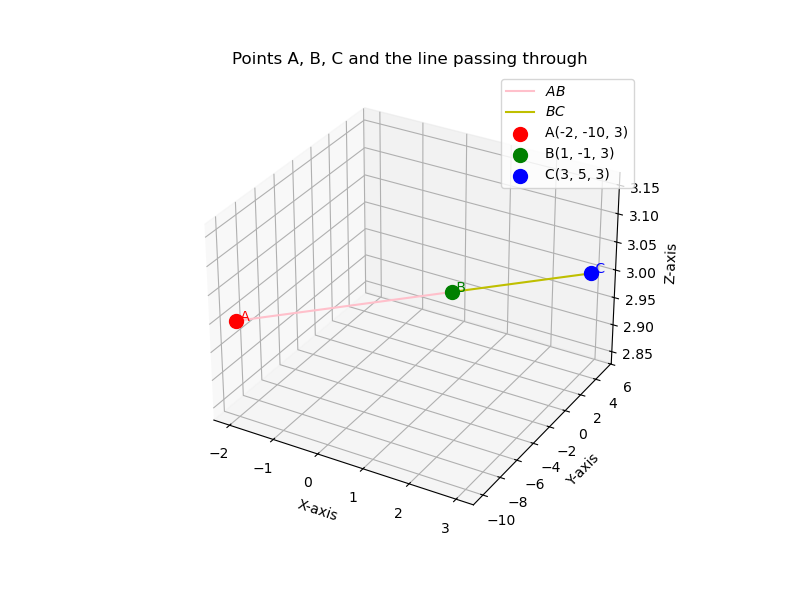
\includegraphics[scale=0.5]{plot}
	\caption*{}
	\label{fig}
\end{figure}
\end{document}
